\documentclass[10pt, a5paper]{article}
\usepackage{ucs}
\usepackage[utf8]{inputenc}
\usepackage[T2A]{fontenc}
\usepackage[english, russian]{babel}
\usepackage{hyperref}
\usepackage{geometry}
\usepackage{graphicx}
\frenchspacing

\begin{document}

\title{Linux и СПО в создании музыки и живом исполнении. Обзор имеющихся программ и ниши применения}
\author{Сергей Васильев\footnote{Таллинн, Эстония, \url{zyxos2@gmail.com}}}
\date{}
\maketitle
\begin{abstract}
The aspects of using Linuz and free software in amateur music creation, sound editing and live performances are reviewed.
\end{abstract}

Ещё несколько лет назад Linux был малопригоден для работы со звуком; за последние годы ситуация значительно изменилась: улучшилась поддержка многих звуковых карт, MIDI-контроллеров и MIDI-интерфейсов, появились новые программы, интерфейс которых изменился в лучшую сторону, что снизило порог вхождения для начинающих пользоваталей. И, несмотря на некоторые всё ещё присутствующие проблемы, сейчас вполне возможно использование решений на базе Linux и СПО в любительской музыкальной деятельности. Применение данных решений имеет ряд преимуществ, одним из которых является низкая стоимость, что немаловажно для начинающих музыкантов. 

Многие начинающие музыканты не обращают внимания на Linux из-за недостаточной информированности, и очень часто для выполнения простых задач прибегают к применению программного обеспечения, возможности которого на порядок превышают потребности, что приводит к нерациональному расходу денежных средств или к незаконному использованию коммерческих приложений. Имеющейся на данный момент программной базы и поддержки оборудования достаточно для выполнения основных задач. 

В таблице приведены категории и некоторые программы, которые, после сравнительного анализа, были отобраны как наиболее подходящие для использования в сетапе для демонстрации.

\begin{figure}[ht]
\centering{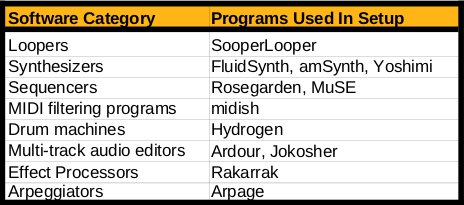
\includegraphics[width=8cm]{13_abstract.jpg}}
%\label{pic:fl1}
\caption{Приложения по категориям}
\end{figure}

\end{document}
